% Шаблон для отчетов по ВКР в СПбГЭТУ "ЛЭТИ"
% Ефремов М.А. 2018г
\documentclass[oneside,14pt]{book}

%=== Настройка кодировок, шрифта и языка
\usepackage[utf8]{inputenc}
\usepackage{extsizes}
\usepackage[main=russian, english]{babel}
\usepackage[T2A, T1]{fontenc}
%\DisemulatePackage{setspace}
\usepackage{setspace}           % Интерлиньяж
\usepackage{geometry}           % Разметка документа
\usepackage{indentfirst}        % Красная строка с первого предложения
\usepackage{titlesec}	        % Форматирование заголовков
\usepackage{titletoc}           % Форматирование содержания
\usepackage{fontspec}           % Установка шрифта для XeLaTeX

%=== Таблицы
\usepackage{tabularx}	        % основной тип таблиц, выравнивание по ширине
\usepackage{longtable}	        % для таблиц, не вмещающихся на одну страницу
\usepackage{multirow}	        % для разбиения ячеек на несколько строк
\usepackage{multicol}	        % на несколько колонок

%=== Работа с формулами
\usepackage{amsmath}            % Набор пакетов, сильно расширяющих возможности по набору формул
\usepackage{amssymb}            % добавляет специфические для русских статей мат. символы вроде \leqslant
\usepackage{amsthm}	            % добавляет окружения для теорем и лемм	
\usepackage{mathtools}          % номера только для тех формул, на которые есть ссылки в тексте

%=== Разное
\usepackage{graphicx}           % Работа с изображениями
\usepackage[unicode]{hyperref}  % Работа с гиперссылками
\usepackage{pdflscape}          % Панорамное расположение страниц
\usepackage{ragged2e}           % Для установки --
\usepackage{microtype}          % -- осустствия переносов
\usepackage{color}				% Использование цветов (нужно для \todo)
%=== Разметка документа
\geometry{
	a4paper, 
	top = 2cm,
	bottom = 2cm,
	left = 3cm,
	right = 1cm,
	%includeheadfoot,
	%asymmetric
}
%=== Форматирование текста
%%%% Междустрочный интервал 1.5 строки
\onehalfspacing		
\linespread{1.43}
%%%% Отступ красной строки - 1.25см
\setlength{\parindent}{1.25cm}	
%%%% Шрифт Times New Roman
\setmainfont{Times New Roman}

%=== Заголовки
%%%% Главы
\titleformat{\chapter}[hang]{\normalfont\bfseries\centering\uppercase}{\thechapter . }{0pt}{}
\titlespacing{\chapter}{0pt}{-4ex}{2.5ex}
%%%% Разделы
\titleformat{\section}[hang]{\normalfont\bfseries}{\thesection .  }{0pt}{}
\titlespacing{\section}{\parindent}{0pt}{2.5ex}
%%%% Подразделы
\titleformat{\subsection}[hang]{\normalfont\bfseries}{\thesubsection . }{0pt}{}
\titlespacing{\subsection}{\parindent}{0pt}{2.5ex}
%%%% Подподразделы
\titleformat{\subsubsection}[hang]{\normalfont\bfseries}{\thesubsubsection . }{0pt}{}
\titlespacing{\subsubsection}{\parindent}{0pt}{2.5ex}


%=== Форматирование содержания
%%%% Глубина вложенности содержания 
\setcounter{tocdepth}{1}           % до подразделов
\setcounter{secnumdepth}{3}        % считать тоже до подразделов
%%%% Формат глав
\titlecontents{chapter}
[0.0cm]             				% левый отступ
{}                  				% предваряющий код
{\contentslabel{3.2em}}  			% формат, если заголовок нумерованный
{}                                  % формат, если заголовок НЕнумерованный
{\titlerule*[1pc]{ }\contentspage}  % заполнение \titlerule*[какой длины повторение]{чем} до номера страницы заголовка.
%%%% Формат разделов
\titlecontents{section}
[0em]
{}
{\contentslabel{2.3em}}
{\hspace*{-2.3em}}
{\titlerule*[1pc]{ }\contentspage}

%=== Минимизируем количество переносов
\tolerance = 500
\hyphenpenalty = 20000
\emergencystretch = 2cm

%=== Номера только для тех формул, на которые есть ссылки в тексте
\mathtoolsset{showonlyrefs=true}

%=== Работа с гиперссылками
\hypersetup{
	colorlinks=true,
	urlcolor=blue,
	filecolor=green,
	linkcolor=red
}

%=== Стиль документа
%%%% Номера страниц внизу
\newpagestyle{mystyle}{\setfoot[\thepage][][]{}{\thepage}{}}
%%%% Применить стиль
\pagestyle{mystyle}
%=== Библиография
\usepackage[
	backend=biber,
	bibencoding=utf8,
	sorting=none,
	maxcitenames=4,
	language=auto, % получение языка из babel
	autolang=other, % многоязычная библиография
	style=gost-numeric
]{biblatex}
\addbibresource{bib/bibliography.bib}
%=== Заголовок оглавления - содержания
\addto\captionsrussian{ 
	\renewcommand*\contentsname{\uppercase{Содержание}}
}

\usepackage{csquotes}
\usepackage{lipsum}
\usepackage{enumitem}
\usepackage{rotating}
\usepackage{pdfpages}

\renewcommand{\descriptionlabel}[1]{\hspace{\labelsep}\textit{#1}}
\usepackage{unicode-math}
\setmathfont{XITS Math}
\setlist[itemize]{noitemsep, topsep=0pt}
\setlist[description]{noitemsep, topsep=0pt}
\addto\captionsrussian{\renewcommand{\figurename}{Рисунок}}

\usepackage{mathtext}

\begin{document}
	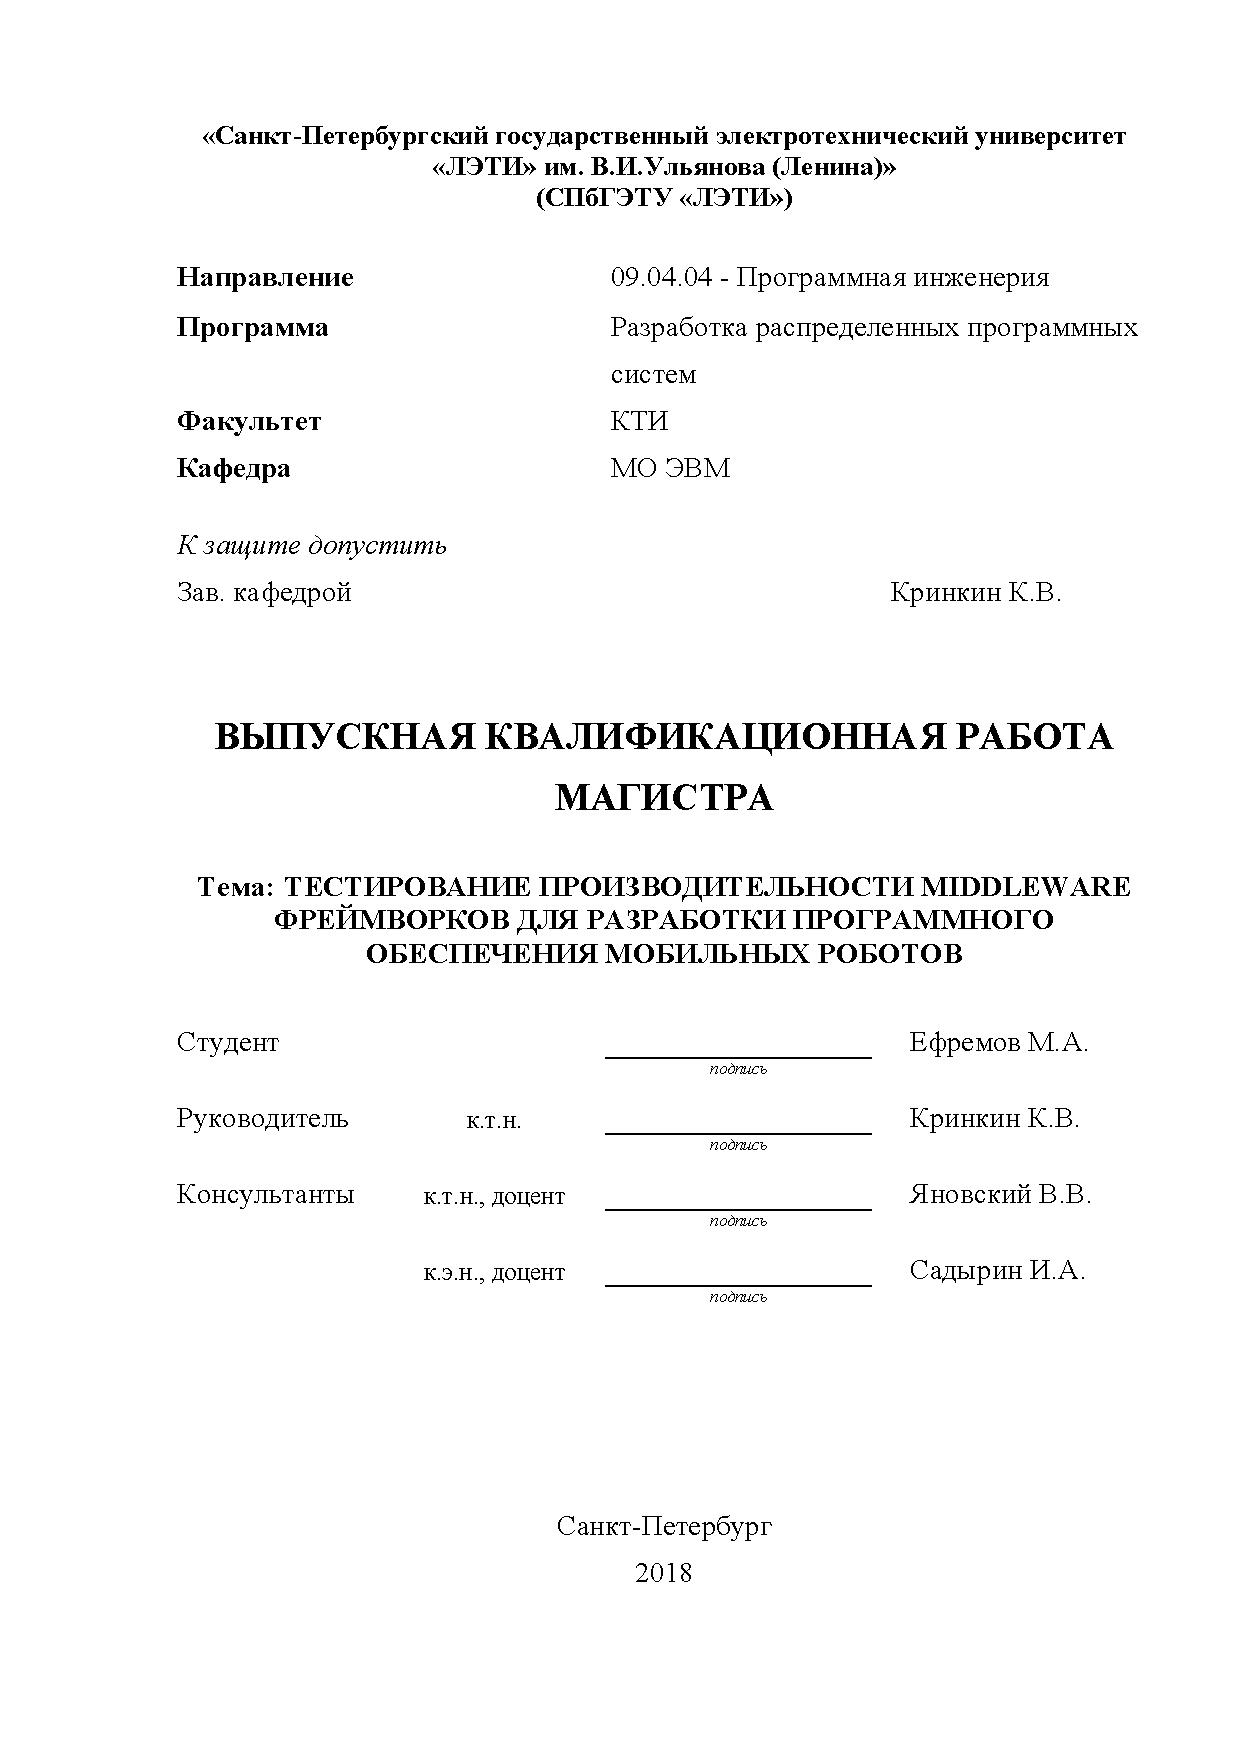
\includepdf[pages=-]{title.pdf}
	\pagenumbering{gobble}
	\chapter*{\todo{Реферат}}
%=== Начало нумерации страниц
\pagenumbering{arabic}
\setcounter{page}{4}
%\leavevmode\newline

\lipsum[1]

Пояснительная записка 00 стр., 00 рис., 00 табл., 00 ист., 00 прил.

КЛЮЧЕВЫЕ СЛОВА И СЛОВОСОЧЕТАНИЯ, НЕ БОЛЕЕ ПЯТНАДЦАТИ, ЧЕРЕЗ ЗАПЯТУЮ

\uppercase{Ключевые слова и словосочетания, не более пятнадцати, через запятую}

Объектом исследования (разработки) являются указать объект исследования или разработки.

Цель работы – кратко (в 2-3 строки) указать цель работы.

Кратко (в 10-12) строк описать основное содержание работы, методы исследования (разработки), полученные результаты.
             % Реферат ! ВНУТРИ НАЧИНАЕТСЯ НУМЕРАЦИЯ !
	\chapter*{Abstract}
Briefly (10-15 lines) the content of graduating work is specified          % Аннотация на английском
	\tableofcontents % Оглавление	
	\chapter*{Определения, обозначения и сокращения}
В настоящей пояснительной записке применяют следующие термины с соответствующими определениями:

\termDef{ОС}{операционная система.}
\termDef{ПО}{программное обеспечение.}
\termDef{ППО}{промежуточное программное обеспечение.}
\termDef{\marm{}}{многоагентное робототехническое программное обеспечение.}
\termDef{API}{Application Programming Interface, интерфейс прикладного программирования.}
\termDef{P2P}{Peer-To-Peer, одноранговая сеть.}
\termDef{URL}{Uniform Resource Locator, единый указатель ресурса.}
\termDef{RTT}{Real-Time Toolkit.}
\termDef{OCL}{ORoCoS Component Library.}
\termDef{GPU}{Graphics Processing Unit, графический процессор.}
\termDef{CPU}{Central Processing Unit, центральный процессор.}
\termDef{ORB}{Object Request Brokers, брокеры объектных запросов.}
\termDef{QoS}{Quality of Service, предоставление различному трафику различный приоритет в обслуживании.}
\termDef{XML}{eXtensible Markup Language, язык разметки.}
\termDef{JSON}{JavaScript Object Notation, текстовый формат обмена данными.}
\termDef{DNS}{Domain Name Service, система для получения информации о доменах в сети.}
\termDef{GUI}{Graphical User Interface, графический пользовательский интерфейс.}       % Определения
	
	\chapter*{Введение}
\addcontentsline{toc}{chapter}{Введение}

Для программирования роботов доступно множество различных версий фреймворков с различными принципами работы, написанные на разных языках программирования и под разные платформы. В связи с тем, что появляются новые разработки, возникают новые задачи для автономных роботов, а так же технологии разработки ПО для них - возникает желание рассмотреть доступные и развивающиеся в данный момент решения и проанализировать с целью установки характеристик производительности и сравнения по полученным параметрам, чтобы разработчики могли обосновывать свой выбор при разработки приложений для автономных роботов. При этом необходимо учитывать как соответствие фреймворков возможным общим критериям (лицензия, статус разработки), так и важным для конкретной области: разработки ПО (программного обеспечения) для роботов. Для выполнения тестирования, следует определиться с тем, какие задачи, выполняемые фреймворком, являются значимыми для производительности системы в целом, какие компоненты системы требуется протестировать.

Для выполнения тестирования требуется использовать корректные инструменты. Тестирование производительности можно выполнять множеством различных методов, технические детали, лежащие в основе драйверов тестирования производительности различны, например, для разных архитектур процессоров. В данной работе рассматривается сравнение ряда фреймворков для автоматизации проведения тестирования производительности.

Составив план тестирования, определившись с тестовыми случаями и реализацией тестовых модулей, требовалось проанализировать полученные результаты и составить сравнительные выводы по итогам тестирования производительности.

\textit{Объектом исследования} в данной работе является множество ППО (промежуточного ПО) для разработки прикладного ПО автономных роботов.

\textit{Предметом исследования} является производительность подмножества наиболее доступного и используемого МАРППО (многоагентного робототехнического ППО).

\textit{Целью исследования} является получение результатов тестирования производительности для наиболее доступного и используемого \marm{}.      % Введение
	\chapter{Обзор предметной области}
\section{Объект и предмет исследования}

\section{Определение и характеристика робототехнического ППО}

\section{Задачи и способы тестирования производительности}

\section{Выводы}  % Обзор предметной области
	\chapter{\todo{План тестирования}}

\section{\todo{Объект тестирования}}
	\subsection{\todo{Факторы влияния на производительность \marm}}
	\subsection{\todo{Разбор методов коммуникации \marm}}
		\subsubsection{\todo{ROS}}
		\subsubsection{\todo{YARP}}
		\subsubsection{\todo{MIRA}}
		\subsubsection{\todo{OROCOS}}

\section{\todo{Описание тестовых случаев}}

\section{\todo{Реализация}}
	\subsection{\todo{Создание тестового окружения}}
	\subsection{\todo{Используемое API Google benchmark}}
	%\subsection{Детали реализации тестовых случаев}
	\subsection{\todo{Автоматизация тестирования и обработки результатов}}
		\subsection{\todo{Архитектура}}
		\subsection{\todo{Реализация}}
		\subsection{\todo{Примеры работы}}
		\subsection{\todo{Тестирование}}

\section{\todo{Выводы}}
  % План тестирования
	\chapter{\todo{Результаты тестирования}}
\section{\todo{Характеристики тестируемого окружения}}
	Тесты проводились на следующей аппаратной конфигурации:
	\begin{itemize}[noitemsep]
		\item 8 процессоров Intel Xeon E5-2580 2.4 ГГц;
		\item 64 Гб оперативной памяти.
	\end{itemize}
	Операционная система: Ubuntu 16.04. Для тестирования был установлен Docker версии \todo{версия}.
\section{ROS}
\label{title:chapter3:ros}
\subsection{Зависимость задержки от определенных факторов}
Разбирая вопрос факторов, влияющих на производительность прикладного ПО для системы ROS, предполагалась важность следующих факторов:
\begin{itemize}[noitemsep]
	\item размер буфера;
	\item количество подписчиков.
\end{itemize}
В ходе тестирования были получены данные, которые позволяют подтвердить или опровергнуть гипотезы о значимости данных факторов для производительности ROS приложений.

\subsubsection{Зависимость от буфера}
Для проверки гипотезы о том, что задержка передачи данных как-либо зависит от размера буфера топика, рассмотрим графики на рисунке \ref{img:ros_buf_l_k}, в которых отражены результаты тестирования задержки передачи данных в системе \enquote{издатель-подписчик} при единственном подписчике, но при разных объемах данных в зависимости  от размера буфера топика.
\img{img/ros/ros_buf_l_k.png}{График зависимостей задержек передачи данных при разных объемах данных в пределах мегабайта от размера буфера топика.}{img:ros_buf_l_k}{\textwidth}
Зависимость примерно линейная и задержка практически никак не зависит от размера буфера топика.

\subsubsection{Зависимость от количества подписчиков}
Для проверки гипотезы о том, что задержка передачи данных как-либо зависит от количества узлов-подписчиков на топик, рассмотрим графики на рисунках \ref{img:ros_subs_l_m} и \ref{img:ros_subs_l_k}, в которых отражены результаты тестирования задержки передачи данных в системе \enquote{издатель-подписчик} при буфере равном 1000, но при разных объемах данных в зависимости  от количества подписчиков.

\img{img/ros/ros_subs_l_k.png}{График зависимостей задержек передачи данных при разных объемах данных в пределах мегабайта от количества подписчиков.}{img:ros_subs_l_k}{\textwidth}
\img{img/ros/ros_subs_l_m.png}{График зависимостей задержек передачи данных при разных объемах данных больше мегабайта от количества подписчиков.}{img:ros_subs_l_m}{\textwidth}

Из графиков видно, что большого влияния количество подписчиков не оказывает на быстродействие системы. Однако, следует заметить высокое, пропорциональное количеству подписчиков, использование памяти. Первоначально тестирование планировалось для 32 подписчиков, но 64 Гб доступной оперативной памяти не хватало даже на 16 подписчиков при объеме сообщений 64 Мб. 


\subsection{Показатели производительности при различных объемах данных}
\subsubsection{\enquote{Издатель-подписчик}}
Разберем графики с зависимостью задержки (секунды) и пропускной способности (мегабайты в секунду) от различных объемов данных, передаваемых в системе. Для рассмотрения берется система из одного издателя, одного подписчика и буфера размера 1000.

\img{img/ros/ros_pubsub_l.png}{График зависимостей задержек передачи данных при разных объемах данных больше мегабайта от количества подписчиков.}{img:ros_pubsub_l}{\textwidth}
\img{img/ros/ros_pubsub_bw.png}{График зависимостей пропускной способности относительно публикующего и относительно принимающего от разного объемах данных.}{img:ros_pubsub_bw}{\textwidth}

На рисунке \ref{img:ros_pubsub_l} видно, что при сообщениях от 16 Мб задержка составляет больше секунды. Это для робототехнической системы является неприемлимым с точки зрения предметной области. Следовательно, ROS не рекомендуется использовать для передачи больших объемов данных, либо учитывать большую задержку при обмене информацией.

На рисунке \ref{img:ros_pubsub_bw} видно, что при сообщениях больше 16 Кб реальная пропускная способность падает из-за роста задержки передачи сообщений. Кроме того, пропускная способность относительно узла-издателя так же падает при передаче сообщений больше мегабайта.

\subsubsection{\enquote{Клиент-сервис}}
\img{img/ros/ros_rpc_l_k.png}{График зависимости времени запроса и ответа при объеме данных до 64 Кб.}{img:ros_rpc_l_k}{\textwidth}
\img{img/ros/ros_rpc_l_m.png}{График зависимости времени запроса и ответа при объеме данных от 256 Кб.}{img:ros_rpc_l_m}{\textwidth}
\img{img/ros/ros_rpc_bps.png}{График зависимости пропускной способности от объема передаваемых даных}{img:ros_rpc_bps}{\textwidth}
\img{img/ros/ros_rpc_pubsub.png}{График зависимостей задержки передачи данных от объема передаваемых даных для разных типов коммуникации в ROS}{img:ros_rpc_pubsub}{\textwidth}
Рассмотрим графики с зависимостью задержки в миллисекундах и пропускной способности в мегабайтах в секунду от различных объемов данных, передаваемых в системе. При рассмотрении клиент-сервисного подхода уникальны следующие детали:
\begin{itemize}[noitemsep]
	\item данные передаются в обе стороны: на запрос и ответ - следовательно объем передаваемых учитывается два раза в полосе пропускания;
	\item имеется возможность измерить время передачи данных в обе стороны.
\end{itemize}

На графиках \ref{img:ros_rpc_l_k} и \ref{img:ros_rpc_l_m} видно, что до 256 Кб задержка отправки ответа незначительна, но при передаче данных от 1 Мб роль задержки ответа резко возрастает.

На графике \ref{img:ros_rpc_bps} видно, что при передаче данных посредством вызова удаленных процедур есть предел полосы пропускания около 650 Мб/с.

Кроме того, интересен график на рисунке \ref{img:ros_rpc_pubsub}, из которого следует, что передача данных при помощи вызова удаленных процедур, при том, что данных фактически при \enquote{сервис-клиент} подходе передавалось в 2 раза больше, задержка у подхода \enquote{сервис-клиент} примерно в 4 раза меньше и приемлима для систем автономных роботов.






\section{\todo{YARP}}
\label{title:chapter3:yarp}
\subsection{Выявленные ограничения}
Несмотря на то, что изначально предполагалось использование объема данных вплоть до 64 Мб, в ходе тестирования было невозможно отправить данные от 1 Мб. Тестирование либо прерывалось с сигналом \textit{Segment Fault}, либо длилось слишком долго. Тестирование прерывалось примерно спустя 15 минут, если управление не переходило к следующему тесту. Если предположить, что тест из 10 итераций занимает 900 секунд и более, то передача данных в автономной робототехнической системе с полученной задержкой неприемлима.

Кроме того, для гарантии целостности передачи информации при использовании RPC-порта не поддерживается протокол UDP.

\subsection{Сравнение типов портов}
Для сравнения производительности различных типов портов будет использоваться протокол TCP. График на рисунке \ref{img:yarp_ports_l} показывает требуемые зависимости от объема передаваемых данных.
\img{img/yarp/yarp_ports_l.png}{График зависимостей задержек передачи данных для разных типов портов от объема передаваемых данных}{img:yarp_ports_l}{\textwidth}
\img{img/yarp/yarp_ports_bw.png}{График зависимостей пропускной способности для разных типов портов от объема передаваемых данных}{img:yarp_ports_bw}{\textwidth}

Как видно на графике, производительность порта с буфером и без практически не различается с минимальным отставанием порта без буфера сообщений.

Если рассматривать пропускную способность всех типов портов, то график на рисунке \ref{img:yarp_ports_bw} показывает, что все три типа портов имеют низкую пропускную способность, колеблющуюся между 115 и 120 килобайтами в секунду.

\subsection{Сравнение протоколов коммуникации}

Сравним производительность буферизованного порта и RPC-порта с различными доступными для них протоколами.

\img{img/yarp/yarp_protocol_buf_l.png}{График зависимостей задержек передачи данных для буферизованного порта с разными протоколами передачи данных от объема передаваемых данных}{img:yarp_protocol_buf_l}{\textwidth}
\img{img/yarp/yarp_protocol_buf_bw.png}{График зависимостей пропускной способности для буферизованного порта с разными протоколами передачи данных от объема передаваемых данных}{img:yarp_protocol_buf_bw}{\textwidth}
\img{img/yarp/yarp_protocol_rpc_l.png}{График зависимостей задержек передачи данных для RPC-порта с разными протоколами передачи данных от объема передаваемых данных}{img:yarp_protocol_rpc_l}{\textwidth}
\img{img/yarp/yarp_protocol_rpc_bw.png}{График зависимостей пропускной способности для RPC-порта с разными протоколами передачи данных от объема передаваемых данных}{img:yarp_protocol_rpc_bw}{\textwidth}

На графиках \ref{img:yarp_protocol_buf_l} и \ref{img:yarp_protocol_buf_bw} изображены показатели производительности различных протоколов для буферизованного порта. Учитывая, что протокол UDP не гарантирует достижение сообщения получателем и реальная пропускная способность у данного протокола ниже из-за потерь дэйтаграмм, то наиболее стабильным с точки зрения пропускной способности и эффективным по времени передачи данных является использование разделяемой памяти, за что в YARP отвечает фреймворк ACE.

На графиках \ref{img:yarp_protocol_rpc_l} и \ref{img:yarp_protocol_rpc_bw} изображены показатели производительности различных протоколов для RPC-порта. Протоколы TCP и FastTCP показывают одинаково низкие результаты производительности и, как и в случае с буферизованным портом, использование разделяемой памяти предоставляет наибольшую производительность коммуникации между узлами робототехнической системы.






\section{MIRA}
\label{title:chapter3:mira}
\subsection{Различие производительности различных типов модулей}
MIRA выделяется подходом к модулям - узлам распределенной системы. В MIRA модулями являются не исполняемые модули, а объекты классов, полученные при помощи реализации шаблона \enquote{Фабрика объектов} внутри самого фреймворка. В общем случае, каждый модуль - это объект класса с определенным интерфейсом. Все модули компилируются как разделяемые библиотеки. Это позволяет реализовать наиболее быстрое межпроцессное взаимодействие: разделяемая память внутри процесса. 

Кроме того, имеется возможность запускать модули в разных процессах, разработчики реализовывают взаимодействие в данном случае при помощи протокола TCP. Тем не менее, гарантия доставки сообщений отсутствует, т.к. сообщение может быть на момент прибытия в нужный узел \enquote{неактуальным} и будет пропущено. В случае, если модули находятся в разных процессах этот факт очень заметен: в 7 из 90 случаев сообщения в ходе тестирования не были зафиксированы системой тестирования. Этим можно объяснить колебания задержки, измеряемой на получателе. Кроме того, получатель не может формально отличить некорректные сообщения первых итераций тестирования, таким образом результаты, измеряемые на узле-получателе так же имеют дополнительную ошибку в виде первых нескольких измерений для каждого теста.

\subsubsection{Задержка передачи данных}
\img{img/mira/mira_res_i_o_ml.png}{График зависимостей задержек передачи данных внутри одного процесса и между двумя процессами в зависимости от объема передаваемых данных на стороне принимающего.}{img:mira_res_i_o_ml}{\textwidth}

На рисунке \ref{img:mira_res_i_o_ml} показаны графики задержки передачи сообщений. На них четко видно, что реальная задержка передачи сообщений между модулями внутри одного процесса на несколько порядков (порядок 1000 наносекунд внутри одного процесса и 10 миллисекунд в разных) ниже, чем в различных процессах. 

\img{img/mira/mira_res_i_o_sl.png}{График зависимостей задержек передачи данных внутри одного процесса и между двумя процессами в зависимости от объема передаваемых данных на стороне посылающего.}{img:mira_res_i_o_sl}{\textwidth}

При этом, на рисунке  \ref{img:mira_res_i_o_sl} отображен график, из которого следует, что время непосредственно публикации данных на модуле-передатчике внутри одного процесса примерно в $1.5$ раза дольше, чем в разных процессах.

\subsubsection{Пропускная способность}

Пропускную способность стоит рассматривать с учетом времени, которое занимает передача сообщения от передатчика к получателю. Если рассматривать время только на передатчике, то результат будет не соответствовать реальности. 

\img{img/mira/mira_res_i_o_bps.png}{График зависимостей пропускной способности передачи данных внутри одного процесса и между двумя процессами в зависимости от объема передаваемых данных.}{img:mira_res_i_o_bps}{\textwidth}

Как видно из графика на рисунке \ref{img:mira_res_i_o_bps}, пропускная способность передачи данных внутри процесса составляет гигабайты в секунду. Фактически, в случае внутрипроцессного взаимодействия, пропускная способность ограничена лишь доступом к оперативной памяти. В случае же межпроцессной передачи данных, пропускная способность достаточно низкая, около десятков мегабайт в секунду.

\subsection{Производительность различных подходов коммуникации}

\img{img/mira/mira_res_rpc_pubsub.png}{График зависимостей задержки передачи данных для различных подходов коммуникации в зависимости от объема передаваемых данных.}{img:mira_res_rpc_pubsub}{\textwidth}
\img{img/mira/mira_res_rpc_bps.png}{График зависимости пропускной способности передачи данных при удаленном вызове процедуры от объема передаваемых данных.}{img:mira_res_rpc_bps}{\textwidth}

В MIRA, кроме шаблона \enquote{издатель-подписчик}, доступно взаимодействие по шаблону \enquote{сервис-клиент}. Сравнение будет вестись для модулей в разных процессах, поскольку чаще всего стоит задача удаленного вызова процедур у другого процесса.

График на рисунке \ref{img:mira_res_rpc_pubsub} показывает, что при удаленном вызове процедур с увеличением объема данных резко начинает возрастать время на передачу данных. Стоит отметить, что в тестах объем данных передавался в обе стороны: от клиента к сервису и обратно. Тем не менее, это не объясняет стремительный рост времени передачи данных при больших объемах данных.

График на рисунке \ref{img:mira_res_rpc_bps} показывает, что при удаленном вызове процедур виден порог пропускной способности: примерно 22 мегабайта в секунду.
%\section{\todo{OROCOS}}
\section{\todo{Сравнение результатов}}
\section{\todo{Выводы}}  % Результаты тестирования
	\chapter{\todo{Технико-экономическое обоснование}}
\section{\todo{Резюме}}
\section{\todo{Описание продукции}}
\section{\todo{Анализ рынка и сбыта продукции}}
\section{\todo{Анализ конкурентов}}
\section{\todo{План маркетинга}}
\section{\todo{План производства}}
\section{\todo{Организационный план}}
\section{\todo{Финансовый план}}
\section{\todo{Инвестиционный план и стратегия финансирования}}
\section{\todo{Анализ и оценка рисков}}
  % Технико-экономическое обоснование

	\chapter*{\todo{Заключение}}
\addcontentsline{toc}{chapter}{Заключение}

Кратко (на одну-две страницы) описать основные результаты работы, проанализировать их соответствие поставленной цели работы, показать рекомендации по конкретному использованию результатов исследования и перспективы дальнейшего развития работы.        % Заключение
	\clearpage                                  % В том числе гарантирует, что список литературы в оглавлении будет с правильным номером страницы
%\hypersetup{ urlcolor=black }               % Ссылки делаем чёрными
%\providecommand*{\BibDash}{}                % В стилях ugost2008 отключаем использование тире как разделителя 
\urlstyle{rm}                               % ссылки URL обычным шрифтом
\ifdefmacro{\microtypesetup}{\microtypesetup{protrusion=false}}{} % не рекомендуется применять пакет микротипографики к автоматически генерируемому списку литературы
\insertbibliofull                           % Подключаем Bib-базы
\ifdefmacro{\microtypesetup}{\microtypesetup{protrusion=true}}{}
\urlstyle{tt}                               % возвращаем установки шрифта ссылок URL
%\hypersetup{ urlcolor={urlcolor} }          % Восстанавливаем цвет ссылок        % Список использованнх источников
	
	\setcounter{chapter}{0}
%	\addtocontents{toc}{\setcounter{tocdepth}{0}}	
	\begingroup
		\renewcommand\thechapter{\Alph{chapter}}
		\titleformat{\chapter}[hang]{\normalfont\bfseries\centering\uppercase}{Приложение \thechapter . }{0pt}{}
		\titlecontents{chapter}[2cm]{}{Приложение \thecontentslabel . }{}{\titlerule*[1pc]{ }\contentspage}
%		\chapter{Таблицы}
\section{Сравнение фреймворков}
	\begin{table*}[h!]
	\scriptsize
	\centering
	%\def\arraystretch{1.5}
	\resizebox{\textwidth}{!}{
		\begin{tabular}{|l|p{2cm}|p{3cm}|p{2cm}|}
			\hline
			\textbf{НАЗВАНИЕ}     & \textbf{ОТКРЫТЫЙ КОД} & \textbf{НАЛИЧИЕ ПОНЯТНОЙ ДОКУМЕНТАЦИИ} & \textbf{ПОСЛЕДНИЕ ИЗМЕНЕНИЯ} \\ \hline
			ROS          & Да           & Да                            & Недавно \\ \hline
			MIRA         & Да           & Да                            & Недавно \\ \hline
			MOOS         & Да           & Да                            & Недавно \\ \hline
			OROCOS/Rock  & Да           & Да                            & 2016    \\ \hline
			ASEBA        & Да           & Нет                           & Недавно \\ \hline
			YARP         & Да           & Да                            & Недавно \\ \hline
			OpenRTM-aist & Да           & Нет                           & 2016    \\ \hline
			URBI         & Да           & Нет                           & 2016    \\ \hline
		\end{tabular}
	}
	\caption{Соответствие найденного робототехнического ППО выделенным в разделе \ref{title:chapter1:mars_criterias} критериям (часть 1)}
	\label{tab:chapter1:mars_solutions_1}
\end{table*}

\begin{table*}[h!]
	%\small
	\centering
	\def\arraystretch{1.2}
	\resizebox{\textwidth}{!}{%
		\begin{tabular}{|l|l|p{4.2cm}|p{3.8cm}|}
			\hline
			\textbf{НАЗВАНИЕ}     & \textbf{АРХИТЕКТУРА}   & \textbf{ИНСТРУМЕНТЫ МОНИТОРИНГА} & \textbf{ПОДДЕРЖКА ЯП} \\ \hline
			ROS                   & Гибридная              & Да                      & C++, Python               \\ \hline
			MIRA                  & Децентрализованная     & Да                      & C++, Python, JavaScript   \\ \hline
			MOOS                  & Централизованная       & Да                      & C++, Java                 \\ \hline
			OROCOS/Rock           & Гибридная              & Да                      & C++, Python, Simulink     \\ \hline
			ASEBA                 & Распределенная         & Да                      & Собственный язык          \\ \hline
			SmartSoft             & Распределенная         & Да                      & C++                       \\ \hline
			YARP                  & Децентрализованная     & Да                      & C++, Python, Java, Octave \\ \hline
			OpenRTM-aist          & Гибридная              & Да                      & C++, Java, Python         \\ \hline
			URBI                  & Централизованная       & Да                      & C++, Java, urbiscript     \\ \hline
		\end{tabular}
	}
	\caption{Соответствие найденного робототехнического ППО выделенным в разделе \ref{title:chapter1:mars_criterias} критериям (часть 2)}
	\label{tab:chapter1:mars_solutions_2}
\end{table*}
		\chapter{Исходный код Docker-файлов}
\label{application:dockerfiles}
\lstinputlisting[language=bash, caption=ubuntu-dev:latest, label=application:dockerfiles:ubuntu-dev]{src/dockerfiles/ubuntu-dev}
\lstinputlisting[language=bash, caption=ubuntu-ros:latest, label=application:dockerfiles:ubuntu-ros]{src/dockerfiles/ubuntu-ros}
\lstinputlisting[language=bash, caption=ubuntu-yarp:latest, label=application:dockerfiles:ubuntu-yarp]{src/dockerfiles/ubuntu-yarp}
\lstinputlisting[language=bash, caption=ubuntu-mira:latest, label=application:dockerfiles:ubuntu-mira]{src/dockerfiles/ubuntu-mira}
\lstinputlisting[language=bash, caption=ubuntu-orocos:latest, label=application:dockerfiles:ubuntu-orocos]{src/dockerfiles/ubuntu-orocos}
		\chapter{Исходный код}
\section{Анализатор результатов тестирования}
\label{application:analyser}
\lstinputlisting[language=python, caption={Merger.py}]{src/merger.py}
\section{Библиотека бенчмарк-тестирования}
\label{application:lib}
\lstinputlisting[language=C++, caption={Benchmark.h}]{src/Benchmark.h}
\lstinputlisting[language=C++, caption={BenchmarkKeeper.h}]{src/BenchmarkKeeper.h}
		\chapter{Примеры файлов конфигурации}
\section{Файл конфигурации исходных json-файлов}
\label{application:config:merge}
\lstinputlisting[language=xml]{src/merge_config.xml}

\section{Файл конфигурации rmarkdown отчета}
\label{application:config:rmd}
\lstinputlisting[language=xml]{src/rmd_config.xml}
	\endgroup
	
\end{document}